\documentclass[10pt]{article}
\usepackage[polish]{babel}
\usepackage[utf8]{inputenc}
\usepackage[T1]{fontenc}
\usepackage{graphicx}
\usepackage[export]{adjustbox}
\graphicspath{ {./images/} }
\usepackage{amsmath}
\usepackage{amsfonts}
\usepackage{amssymb}
\usepackage[version=4]{mhchem}
\usepackage{stmaryrd}

\title{POLITECHNIKA \\
 GDANSKA \\
 CENTRUM MATEMATYKI }

\author{}
\date{}


\begin{document}
\maketitle
\section*{OD SZKOLNIAKA DO ŻAKA}
\section*{klasy 5 i 6 szkoły podstawowej}
rok szkolny 2021/2022

\section*{Zadania - etap II}
Zadanie 1. Bok kwadratu ABCD wynosi 5 cm . Oblicz pole trójkąta CEF wyciętego z kwadratu BEFD.\\
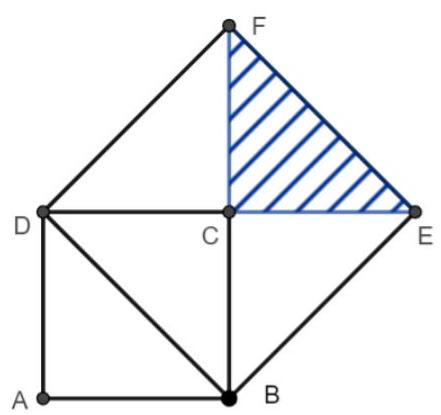
\includegraphics[max width=\textwidth, center]{2024_11_21_c6672992d8aeb6aa1085g-1(1)}

Zadanie 2. 6 zeszytów 32-kartkowych kosztuje tyle co 3 zeszyty 100-kartkowe. O ile procent droższy jest zeszyt 100-kartkowy od 32-kartkowego, jeżeli ten 32-kartkowy kosztuje 2,75 zł?

Zadanie 3. Oblicz bez użycia kalkulatora, przedstawiając wszystkie obliczenia, następującą sumę: \(\frac{1}{15}+\frac{1}{35}+\frac{1}{63}+\frac{1}{99}+\frac{1}{143}+\frac{1}{195}+\frac{1}{255}+\frac{1}{323}\). (Wskazówka: \(\frac{1}{15}=\frac{1}{3 \cdot 5}=\frac{1}{2}\left(\frac{1}{3}-\frac{1}{5}\right)\) )

Zadanie 4. Kasia zalała kawą plan swojego nowego mieszkania, tracąc w ten sposób część wymiarów. Te, które pozostały, widoczne są na planie. Ile pełnych paczek terakoty na podłogę łazienki musi kupić Kasia, jeżeli w jednej paczce mieści się 1,2 m² płytek a powierzchnia całkowita mieszkania wynosi \(60 \mathrm{~m}^{2}\).\\
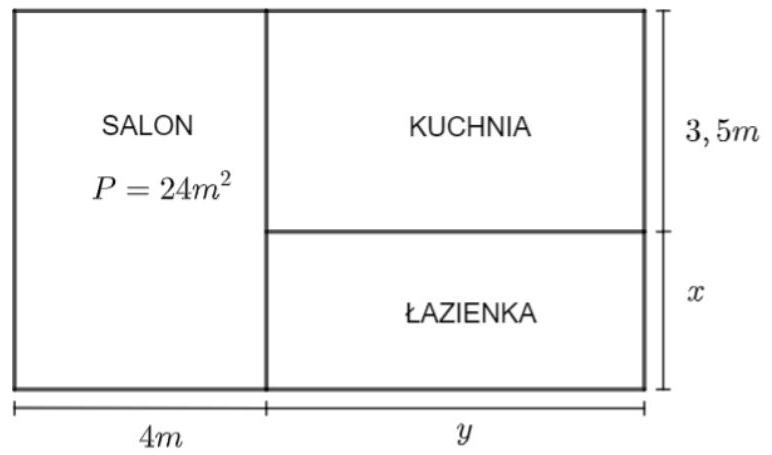
\includegraphics[max width=\textwidth, center]{2024_11_21_c6672992d8aeb6aa1085g-1}

Zadanie 5. Pod jabłonią Antek znalazł jabłka. Wziął \(\frac{1}{11}\) z leżących jabłek, a jego brat Wiktor tylko 4 jabłka. Razem mieli \(\frac{1}{9}\) leżących pod jabłonią jabłek. Ile jabłek zostało pod jabłonią?


\end{document}